\documentclass[conference]{IEEEtran}
\usepackage{color}
\usepackage[color]{coqdoc}
\usepackage{graphicx}
\usepackage[justification=centering]{caption}

\hyphenation{op-tical net-works semi-conduc-tor}

\begin{document}
%
% paper title
% can use linebreaks \\ within to get better formatting as desired
\title{Foundations for Multi-Property Systems Engineering}

\author{
\IEEEauthorblockN{Kevin Sullivan, Chong Tang, Ke Dou, Koleman Nix}
\IEEEauthorblockA{
Department of Computer Science\\
University of Virginia\\
Charlottesville, Virginia 22904-4740\\
Email: \{sullivan, ctang, kdou, jkn3wn\}@virginia.edu
}
%	\and
%	\IEEEauthorblockN{Barry Boehm}
%	\IEEEauthorblockA{
%	Department of Computer Science\\
%	University of Southern California\\
%	Los Angeles, California 90089-0781\\
%	Email: boehm@sunset.usc.edu
%	}
}


% make the title area
\maketitle
\begin{abstract}
The purpose of engineering is to create value for the stakeholders in a system. Value in turn arises from a combination of diverse system {\em properties} and stakeholder {\em value propositions}. A major problem in engineering today is that we are generally unable to effectively ascertain, communicate and reason about, balance, specify, and assure many value-critical system properties. Decades of effort to develop and promulgate informal definitions of properties and relationships among them have not converged to broadly accepted or particularly useful results. We offer a new approach to this problem: a method of representing generalized theories of system properties and relationships in the language of mathematics, logic, and computation, in a manner that enables such theories rapidly to be automated and deployed for evaluation so that they can quickly evolve into {\em validated} forms that are accessible to a broad community. We employ the constructive logic of the Coq proof assistant---which has proven to be useful for formalizing mathematics, logics, languages, computations, and proof checking---for this purpose. Theories expressed in this form provide for both {\em definition} and {\em specification} of properties, in both general and system-specific forms, and for the construction and checking of key elements of {\em property and value assurance cases} for complex systems. We offer evidence that this approach has the potential as a breakthrough advance in systems and software engineering, including but not limited to the not only the formalization but reconciliation and integration of two notable and previously competing, informal theories, and a concrete example of its application to a cyber-physical-human (CPH) system for building automation.
\end{abstract}

\IEEEpeerreviewmaketitle

% The system engineering research community has been working on defining system qualities for many years. However, we still do not have shard understanding of, neither great ability to engineer them. Moreover, it is very difficult to make trade-offs among system qualities. These problems are rooted in the facts that we just have weak engineering foundations and weak scientific foundations. Most researches in this area has been informal and qualitative. Theories are expressed informally with natural language, tables, and graphics. We just have weak basis for automation, dissemination, testing, validation, and adoption and evolution of basic concepts, methods, and tools. Besides, we just have weak understanding the natural of assurance, in particular in understanding the role and interpretation of evidence and the relationship between inductive and deductive reasoning in system quality assurance.

% Some, such as safety, are better understood than others, and we do have the means to manage certain properties in isolation, but we lack the means to manage the full range of critical properties, and the interplays among them, across the system lifecycle for complex cyber-physical-human (CPH) systems.

\section{Introduction}
The value of a system arises from the combination of system properties stakeholder value propositions. Value-critical properties, which are sometimes called {\em system qualities}, {\em quality attributes} or just {\em ilities}, range from physical and cyber system functionality, to dependability, usability, flexibility, affordability, and others. This paper focuses on gaps in knowledge and method that, for complex systems, make it hard to define and specify many properties and to provide assurance across the lifecycle that a system will have a  {\em value-producing stakeholder-effective balance of the full set of system properties} needed for a system to be successful. 

In systems engineering, in general, as in software engineering, in particular, significant research and development effort has been devoted to the issue of requirements. Yet requirements for system {\em quality attributes} are generaly either not specified at all, or are specified in terms that are vague and unclear terms and consequently not a basis for rigorous development~\cite{bosch-isa99}. 

The basic contribution of this paper is an approach to developing a rigorous, useful, and unified science of property definition, specification, management across the lifecycle, and assurance. We present an instance of the approach and a notional example of its application to a real system. Our analysis suggest that the approach is worth pursuing. Our idea is to develop mathematically, computationally, and logically formal languages and reasoning frameworks to address these needs. 

Such a framework has two basic elements. The first is a top-down, generalized means-ends hierarchy of qualities, rooted in {\em value} as the top-level quality, and parameterized by a system type, instance of that type, a stakeholder set, a set of operational contexts, and a set of lifecycle stages. This hierarchy is formalized as a {\em propositional} structure. It implicitly defines higher-level qualities in terms of lower-level ones. It supports tracking of quality requirements and assurance across the lifecycle by making requirements explicit. It supports the logical components of quality assurance cases by establishing a constructive logic framework for producing proofs that higher-level quality propositions are satisfied from proofs that lower-levels propositions are satisfied. The structure both standardizes and partially automates rules for reasoning about the satisfaction of high-level system quality requirements. 

The second key component of our approach is a set of {\em little languages} for articulating detailed and system specific quality requirements at the leaves of the top-level taxonomy, or means-ends hierarchy. The nodes in the taxonomy are very abstract and are meant to apply to a very broad range of cyber-physical-human systems, but they are so general as not to be particularly useful for expressing system-specific requirements. Nor could any single language possibly suffice to express the broad range of quality requirements---general representations of which are given at the leaves of the taxonomic hierarchy, e.g., ranging from usability to security resilience to evolvability, speed of development, physical range, battery life, and maneuverability, and including many more. We thus provide a range of quality-specific {\em little languages} that can be used to formally state specific, detailed quality requirements for particular systems. Our top-down taxonomy is parameterized by what one can view intuitively as containers for system-specific, detailed quality requirements propositions expressed using these quality-specific little languages. 

This approach provides the engineering with a general-purpose framework for tracking a comprehensive range and hierarchy of system quality requirements, but one that is ultimately rooted in detailed, quality-specific, and system-specific requirements linked at the leaves of the general-purpose hierarchy. It is entirely up to the engineer to elaborate detailed specifications to the level that is appropriate in a given environment. In terms of assurance, what one must ultimately provide in order to obtain a certificate (formally a proof object) that the top-level value proposition for the system is satisfied are certificates (proof objects) for the low-level quality propositions. In practice this could be done by axiomatic acceptance of the propositions, e.g., on the basis of inductive reasoning from evidence analyzed outside of our framework, or alternatively by deductive reasoning from the system model that is given as a parameter to our framework.  

Our framework builds upon, improves, extends, and synthesizes two notable, previously apparently conflicting, informal approaches to these issues, along with a body of work on assurance cases. The first is recent work of Boehm and Nupul~\cite{}, who proposed an informal means-ends {\em taxonomy} of system qualities. Their work stresses that requirements for any given quality attribute will in general vary across combinations of stakeholders, contexts of operation, and stages of system development and operation. The upshot is that simplistic quality requirements, such as {\em the system reliability must be 99.999\%} are untenable, and must be decomposed into many stakeholder-, context-, and stage-specific subrequirements, e.g., addressing the widely varying notions of reliability across the stakeholder based in a complex system. They also emphasize that there are inherent tradeoffs among system qualities, that these must be understood and managed, and that a framework should support reasoning about tradeoffs. 

The second work that we draw upon is that of Ross et al.~\cite{ross-15}. They start with the thesis a long history suggests that top-down attempts to formulate broadly accepted definitions of quality attribute terms are destined to fail. They thus eschew such attempts and propose that instead one should start by trying to characterize the {\em spaces} of quality requirements statements that are evidently useful in particular broad quality areas, such as changeability, and that one can then classify each statement in such a space as addressing one more more lower-level qualities, such as flexibility, adaptability, or configurability.

Finally, our concept of quality and value assurance draws on rich body of work in the area of assurance cases~\cite{}, mostly safety cases for software-intensive systems, but generalizing to dependability more broadly\cite{}, and ultimately to overall system success~\cite{knight-success-cases}. The challenge that assurance cases address is to present compelling arguments, usually addressed to certification authorities, supported by evidence and analysis, for the likely validity of propositions that given systems are acceptably safe, dependable, or acceptable in some more general way. 

The overall form of reasoning in an assurance case is inductive, insofar as the evidence considered is usually diverse in form and far short of any kind of formal proof. That said, several researchers have argued that deductive reasoning structures play a vital role in assurance arguments. The idea is that one can separate {\em epistemic} reasoning about whether or not to accept certin low-level propositions in an assurance case (axiomatically) based on inductive reasoning, on one hand, from deductive reasoning about the logical consequences of such axioms~\cite{rushby15}. While questions remain about the validity of such a separation of concerns, we nevertheless accept it for our purposes in this work. In a nutshell, our propositional means-ends hierarchy comes with a set of proof rules for constructing proofs of higher-level quality propositions from proofs of lower-level propositions, with lower-level proofs possibly constructed as mere axioms that encoding provisional acceptance on the basis of inductive reasoning done outside of the deductive logic of our quality attribute hierarchy.  

\section{Contributions}

Before presenting technical details of our approach and examples to help clarify their use, we summarize key challenges that we faced and overcame in this work, the solutions to which constitute the main technical contributions of this present work. These challenges were as follows:
\begin{enumerate}
\item to formalize, clarify, and generalize Boehm's informal taxonomy of properties, relationships, and value;
\item to structure a theory to capture Boehm's general concepts while making it specializable to a broad range of systems;
\item to reconcile and integrate Boehm's taxonomy with Ross's {\em semantic basis} approach;
\item to thereby test two specific propositions: (1) the approaches of Boehm and Ross are not competing and incompatible, as some have suggested, but complimentary and synergistic; and (2) integrating them provides a path toward a rich theory that combines a high-level definitional taxonomy with a range of property-specific {\em little languages} to provide a theory that can structure comprehensive engineering of a broad ranges of general system properties that are nevertheless rooted in detailed, system-specific property requirements;
\item to produce a theory that unifies high-level property {\em definition}, system-specific property {\em specification}, and the deductive components of system-specific property and value {\em assurance};
\item to produce a theory with the flexibility to support model-based approaches to formal reasoning about system properties;
\item to produce a ``toy'' example of the application of such a theory to structure requirements for a particular system, to clarify the nature and intent of our work and to test the propositions that our parameterized approach to theory expression enables our generalized top-down taxonomy to be extended with separately defined, system-specific requirements, and that the general top-down taxonomy provides for bottom-up derivation of deductive ``proofs'' as components of assurance cases.
\end{enumerate}

We have addressed and resolved each of these issues.  We have formalized and clarified Boehm's informal taxonomy. We used Coq typeclasses to enable detailed and system-specific property specifications in the form of typeclass instances. We have showed how propositions incorporating property-specific little languages can be integrated into our high-level taxonomy by extending our formalization Boehm's taxonomy with our formalization of Ross's little language for expressing change-related requirements This result shows the approaches to be complementary and synergistic, and that one could further extend this work easily to incorporate little languages for expressing other properties. We are currently working on a little language for expressing security and resiliency properties. Our high-level taxonomy provides a unified approach to defining high-level properties as functions of lower-level properties, comprehensive property specification, and property assurance based on constructive proofs as part of a larger property and value assurance effort. In this paper we do not explore the possibility of using rich system models (carried by system types and values) as a basis for deductive reasoning about properties. Our work provides the flexibility to do so. To date we have not explored this dimension. In particular, it is important to understand that we are {\em not} arguing that one should try, or that we have provided a capability, to prove all required system properties deductively from system models. We are certainly not arguing that Coq is an appropriate formalism for all formal reasoning tasks. A comprehensive approach to formal verification of system properties would require an extensive range of modeling formalisms and verification tools (e.g., SMT solvers, simulators, model checkers, and so forth). 

%separating them from our expression of a generalized property-value means-ends hierarchy, while enabling the integration of the two for purposes of structuring overall specifications and reasoning about assurance. We have used propositional constructs to formalize properties, claims, and proofs, the latter of which are based on axioms interpreted as denoting human judgments that propositions about a system satisfying detailed specifications are valid (based on evidence and inductive arguments external to the theory). We have exploited patterns of using Coq to formalize the syntax and semantics of languages to reinterpret the earlier works of Boehm et al. and Ross et al. in the computational framework of programming languages and semantics. We are relying on the extraordinary expressiveness of this logic to enable us to ``say what we need to say'' across the diverse range of concerns that are sure to arise in the field in which we are working. This paper provides some reasonably compelling evidence, particularly in the ease with which we were able to integrate the previously disconnected works of Boehm et al. and Ross et al. that this approach is one that works.


% A key ingredient of our approach---the {\em secret sauce}, as it were---is our choice of a {\em maximally expressive} formal language in which to formulate our theories.  We have elected to use the languages of the Coq constructive logic proof assistant~\cite{coq} for our purposes.


%Among the range of non-functional properties, enormous research efforts have been made in such areas as safety, reliability, and human factors. We do have significant scientific and engineering knowledge and capability in these areas. While much does remain to be done within these {\em vertical} properties domains\footnote{In safety, for example, the essential nature and practical construction and use of safety assurance cases remain unresolved.}, extant knowledge does provide practical capabilities to engineer for and to practically assure some of these properties in isolation.

%pt of innovation experiment systems with the use of rigorous formal specification and software synthesis using constructive logic proof assistant technology. We refine and express quality theories using the highly expressive language of the Coq proof assistant, which is capable of unified treatment of mathematical, computational, and logical concerns. We use synthesis from such specifications to support continuous deployment of web-based software implementations of the concepts embodied in such theories, and user-driven testing based on such tools to drive theory testing, evolution, and validation. Elements of the specific framework that we are constructing include a hierarchy of qualities and relationships parameterized by stakeholders, contexts, and system operational stages, based on recent work by Boehm \cite{Boehm:ontology}; quality-specific specification languages for expressing detailed requirements (based on recent work by Ross and Rhodes \cite{Ross:semantic}); and a novel integration of the distinct, previously conflicting theories underlying these two efforts. We present our overall approach and illustrate its application with an example system for home automation. Our goal of this work is to create, validate, promulgate, evaluate, evolve, and drive real-world use of practical concepts, methods, and tools for addressing the engineering problems that we outlined above. The overall contribution of this work is a novel, rigorous, and promising new approach to developing, promulgating, testing, evolving, and validating the scientific theory that is needed to underpin rigorous new approaches to comprehensive system quality engineering.

The rest of this paper is structured as follows. {\em Provide a roadmap here.}


\section{Example}
Consider as an example an advanced home automation system. Purposes might include (1) providing comfort and convenience to occupants to improve quality of life while visibly reducing resource utilization, saving money over time, and reducing environmental impacts; (2) enabling occupants to understand their costs and impacts relative to others; (3) interoperating with emergency systems to anticipate and mitigate risks from fire, crime, and weather; (4) providing sensor data to smart city services ranging from disaster response to resource pricing and policy making; (5) providing a sustainable competitive advantage and profits to the manufacturer.

At the outset of an effort to develop and market such a system, its producer and investors will want reasonable assurance, given their risk and reward preferences, that the system as currently designed will likely achieve its stated purposes. When the system is ready to put into large-scale production, a stronger degree of assurance will be desired. Once the system is finally operating, an even higher level of assurance becomes possible, based on data collected from the system itself as it operates in the deployment environment.

Our use of the term {\em system} so far begs the question, {\em what is the system? What is the system boundary?} While one might assume that the system is the technology that that will be installed in the home---the device, as it were---this answer is too narrow. To answer this question effectively, one should start with the question, {\em What properties are required to achieve the purposes of the initiative and what elements must be managed to produce those properties?} 

For example, the combination of required {\em affordability} to home occupants and {\em profitability} for the producer dictate that the monetary and temporal costs of both system design and manufacturing must be managed. Design and manufacturing processes thus come within the system boundary. Similarly, if the system must reasonably assure the {\em privacy} of occupant data (with implications for {\em safety}), then the software design process, including such factors as developer competence and the use of appropriate tools and methods, enters into consideration. In general, both the artifact being produced (often called {\em ``the system''}) and the processes and mechanisms by which it is produced (sometimes called the {\em meta-system}) are within the system boundary for purposes of this work.

For such a system to be successful, i.e., to achieve its full range of stated purposes, it must possess a broad range of functional and non-functional system properties. We highlight a few for purposes of illustration and to set up the example that we will use for the remainder of this paper.

Such a system must have physical and cyber {\em functionality} properties, such as the ability to sense occupancy; to manage electrical devices; to authenticate users; and to interact with other systems. The system must have {\em usability} and {\em accessibility} properties to enable safe and effective use by people of varying ages, physical, and cognitive abilities. It must be {\em endurable}, to continue operating over a long periods (decades) in the face of wear and tear to physical and computational components. It system must be {\em scalable}, e.g., to handle data as thousands then millions then tens of millions of devices are sold. It might need to be {\em versatile}: e.g., re-purposable to support health monitoring of elderly residents. It will have to be {\em interoperable} and {\em dependable}: reliable (few failures), available (little downtime), safe (no significant hazards to occupants or others), secure (e.g., hackers cannot learn about occupancy to plan break-ins), and so forth. To be economically {\em sustainable} its design and the installed devices will have to be {\em modifiable} to affordably accommodate changing technology and market conditions. It will have to be {\em configurable} to many different environments. It will have to be {\em adaptable} to the patterns of life of individuals and families.

%Complicating matters are the complex interplays among such properties, arising from several sources. First, design decisions that might be made in the interest of one property can have both positive and negative impacts on other properties~\cite{beohm}. For example, adding device redundancy to improve reliability and endurability will increase costs reducing affordability and profitability. Adding strong authentication for security will reduce usability. Adding web service interfaces for interoperability produces security risks. 

%Second, success-critical stakeholders often have strongly varying preferences impacting on system properties. The stakeholders in such a system are diverse. Here they range from the manufacturer's employees and owners, to home occupants, to public agencies (e.g., fire departments), to the broad public (for improved public safety and environmental impact mitigation). Homeowners might prefer low cost of ownership, a short break-even period, ease of use, reliable functionality, and personal privacy. The manufacturer might prefer low cost of design and production and the ability to sell add-on services and devices once the base device is installed. 

%As Boehm has argued~\cite{boehm}, the ability to manage such a major challenge that designers of such cyber-physical-human systems face

\section{The problem}

The problem we face as systems engineering researchers and practitioners is that nature of such properties and the roles they play in creating value for stakeholders are complex, poorly understood, and poorly managed across the system lifecycle. The end result is that our society and industry experience far too many costly and dangerous project and operational system failures. 

\subsection{Facets}
This complexity has numerous facets. First, the space of properties is not flat but organized in a means-ends hierarchy. Higher properties arise from and are supported by lower-level properties. For example, dependability~\cite{Laprie:dependability} arises from reliability, availability, safety, and security. Security, arises from confidentiality and integrity, and supports privacy. We lack a consensus understanding of such means-ends hierarchies sufficient to support systematic engineering of properties across diverse systems.

Second, stakeholders have varying, role-specific, often conflicting preferences regarding properties~\cite{Boehm:ontology}. Not only do different stakeholders generally prefer different tradeoffs; but at a deeper level they may have different interpretations of, and, {\em ipso facto}, different preferences for, given properties. Someone responsible for process compliance will be concerned with the reliability of the prescribed development process, for example, while the test pilot is likely to be more directly concerned with the reliability of the breathing apparatus. Similarly, the project manager responsible for controlling project cost might be in conflict with the engineer who wishes to add redundancy, and thus cost, to achieve a desired reliability property.

Third, properties can become coupled in complex ways through design decisions~\cite{suh, boehm-cser-2015-paper}. For example, a decision to modularize a system to improve changeability can degrade affordability, as a decision to provide single-sign-on to a systems of systems to improve usability can degrade security. Designing architectures that achieve tradeoffs that are consistent with the value propositions of diverse stakeholders remains more art than science, and a not very reliable art.

Fourth---and central to this paper---with the exception of certain well studied properties such as dependability, we lack the basic knowledge and methods required to engineer system properties: even in isolation, not to mention in combination with many other properties. Our gaps in understanding include the lack of agreement on precisely what phenomena we are talking about when we use property terms, such as {\em resilience} or {\em flexibility}, lack of agreement on the precise meanings of the terms often used to refer to properties, lack of agreement on which terms to use to refer to given properties, lack of understanding of means-ends relationships among (ill-defined) properties~\cite{Ross:semantic}, and a lack of means for reasoning about tradeoffs and ultimately stakeholder value. We lack sufficiently precise, shared, and validated scientific knowledge, languages, models, meanings, methods, and tools to manage the full range of system properties across the lifecycle with rigor appropriate to the engineering of complex, costly, often critical systems. 

\subsection{Consequences}

This problem is deeply harmful. It produces one unexpected, but ultimately predictable, and costly, project or system failure after another. Projects are cancelled after consuming billions of dollars. Others overrun their budgets and delivery deadlines by huge margins, or deliver systems with far less capability than expected. Operational failures put people, resources, and the environment at risk. In some cases, system developers {\em game the slack} left by poor definition and management of system properties, e.g., by building a system with less than the property required, knowing that absent clear, verifiable requirements, a buyer will unlikely prevail in a dispute. The routine shortchanging of security properties in many infrastructure components is one example of a failure to manage important system properties in the public interest. 

\subsection{Causes}

We believe that these problems are largely traceable to weaknesses in the science and in methods used to produce the science underlying current concepts, methods, and tools for managing system properties across the lifecycle. We focus on two specific issues.

The first is an inadequate focus on {\em multi-property, value-driven} systems engineering. Property-oriented research has generally focused on achieving individual system properties in isolation. To the extent that we have scientific and engineering disciplines addressing system properties, they are largely stove-piped. We have separate disciplines of dependability and usability engineering, for example, but little in the way of a science or engineering discipline of multi-property requirements analysis, specification, tradeoffs, value, and value {\em assurance.} While such work remains relevant, the bigger challenge now is to achieve acceptable balances among many competing system properties. 

Second, research and practical methods in this area on the whole have long been lacking in rigor and precision. Concepts are all too often expressed in informal, natural language, sometimes with helpful auxiliary diagrams and tables, for example, rather than in rigorously mathematical, computational, and logical forms that can support rigorous engineering analysis and automation. The limits of such an ``intuitive'' approach are now being reached. Ross et al.~\cite{Ross:semantic}, for example, have documented how decades-long and ultimately unproductive {\em property definition wars} that have left us with a Tower of Babel of mostly vague definitions for expressing and reasoning about system properties.

\section{Vision}

We propose an approach to address these problems rooted in a vision of mathematically, computationally, and logically precise, generalized, and ultimately {\em validated}, theories of system properties, value, and assurance. By a {\em theory} in this context, we mean a formal and general mathematical structure that is hypothesized to usefully model the reality of concerns regarding properties, tradeoffs, and value in real systems engineering projects, with evidence generated by testing of the theory against reality that this is the case. Before getting to details, we further detail some of the desirable properties of such a theory.

(1) It should be expressed in a formal (mathematical, logical, computational) notation, precise and unambigous, and capable of concise, abstract representation of classes of complex structures, including parameterized propositions about properties of systems and corresponding proof structures. (2) It should preserve, express, and extend our best informal understanding of properties and related issues. (3) It should be general in covering a broad range of properties and being applicable to a broad range of systems. (4) It should connect properties to stakeholder value (the ultimate property of any successful system). (5) It should address our lack of consensus definitions of system properties by promulgating general definitions of some properties as functions of others in a formal means-end hierarchy. (6) It should be straightforward to {\em extend} and {\em specialize} to support the representation of detailed, system-specific and domain-specific properties. (7) It should support the deductive aspects of property and value assurance. These include deduction of proofs that higher-level properties hold from axiomatically accepted proofs of propositions about low-level properties (where axiomatically accepted proofs are generally based on inductive reasoning from evidence outside of the formal theory) and formal derivation properties from formal system models. (8) A theory should be extensible to support the representation of and reasoning about tradeoffs among properties, e.g., as induced by design decisions represented within formal system models. (9) As with any scientific theory, its validity should be tested, evolved, assessed against the needs of practicing researchers and practitioners. Tenth, it should provide a conceptual foundation for practical and effective systems and software engineering tools and methods.

\section{Approach} 

Our approach  combines several basic elements.  

First, we formalize, thus clarify, and leverage and extend key extant but informal and imprecise works that address the problem we are addressing. The first is recent work of Boehm et al.~\cite{boehm}, which argues that property preferences do, and thus specifications should, vary by stakeholder, context of system operation, stage of development, and in other dimensions.  The paper then presents a stakeholder-value-sensitive means-ends hierarchy, or {\em taxonomy}, of system properties. We formalize this work in this paper. The second work is is a recent paper by Ross~\cite{}  that first characterizes the long history of a failure of research community to settle on definitions of property teams, and that then offers a so-called {\em em semantic basis} approach to defining property-oriented terms. The key idea in this work is that one can define little languages to express requirements within a family of (e.g., changeability-related) properties, and then classify statements in this language as pertaining to more specific sub-properties (e.g., to flexibility, adaptability, or modifiability). We presented an analysis and formalization of his work in a recent paper~\cite{sullivan-cser15}. We also draw on the larger body of work on property assurance cases (usually dependability, and often specifically safety assurance)~\cite{}. The very recent work of Rushby~\cite{} in particular tends to support the idea that we can embed a formal logical structure, and use deductive reasoning, within a broader approach to assurance that requires inductive reasoning in the presence of undercertainty from imperfect, incomplete, and incommensurable forms of evidence. 

Second, we not only formalize, clarify, and extend the Boehm and Ross models, but reconcile and integrate them. We claim that this result yields a new path forward toward a rich library of property-specification templates and languages for property definition, system specification, and value assurance. The key observation is that Ross's little, property-specific languages can be used to {\em flesh out} system-specific instances of our formalized version of Boehm's high-level property taxonomy. Our key insight in this area was that we could parameterize our formalization of Boehm's taxonomy with what one can think of as containers for propositions about low-level properties. These containers can be filled with propositions stating that a given system satisfies system-specific property requirements expressed in a language {\em such as the one} that Ross et al. envisioned. It will be clear that there is no restriction on the range of languages that can be used in this manner.  Very different little languages might be used for usability requirements than for changeability or dependability requirements, for example. 

Third, we adopted a highly expressive formal language in which to express our theory. No single narrow formalism---e.g., finite state machines, relational algebra, logic programming, Petri nets, for example---can feasibly express the range of concerns that must be addressed when on seeks to integrate across a huge diversity of properties, system types, forms of reasoning, forms of evidence, and system stakeholders. We thus traded away automated reasoning in the general case for extreme expressiveness. 
We chose to use constructive (or intuitionistic) logic (also called type theory), as realized in the Coq proof assistant~\cite{coq}, to formalize our theory. 

We needed a language that could formally and readily express properties of cyber-physical systems, diverse system models, a variety of little property specification languages, propositions and deductive proofs objects for use in assurance cases, and more. Coq's higher-order, polymorphic, and dependent type system fits the bill. The recent work of the Fields medalist, Voevodsky, and others has show Coq to be suitable for formalizing deep mathematics. It has been used to represent, reason about, and compute using computational languages~\cite{pierce} ranging from high-level imperative and concurrent languages to assembly code. It is used to specify and to reason about algorithms and data structures, and in work that aims to produce proofs of security properties in complex software~\cite{}. Coq's support for formalizing both mathematical/computational content and logical propositions and proofs is critical. We formalize of Boehm's taxonomy in large part as a set of parameterized propositions about given systems having specified properties, and we roll up such proofs into larger proofs of higher-level properties. Coq also supported automated extraction of computational content into code written in ordinary programming languages, such as Scala, Haskell, and OCaml.

Fourth, we formalize Boehm's overall taxonomy as a Coq typeclass, parameterized by a system type, system instance, set of stakeholders, a set of operational contexts, and a set of propositions that all system properties are certified as present. Instantiating this typeclass requires proofs that these propositions are true. We expect that in most cases, proofs of low-level properties will be given as axioms reflecting human judgments that such properties are present. That said, our formalization admits the definition of rich system models and formal derivation of proofs of properties from such models. 

Coq typeclasses support the definition of what amount to classes of algebraic structures, such as groups, rings, and fields. Such structures are parameterized by types, values, operations, and invariants that must be proven to hold.  Consider the group of the integers mod k under addition, for example. It is an instance of the group typeclass, where the carrier set (type) is the integers mod k, the identity element is zero, the binary operator is plus mod k, the inverse function is the usual one for this group, and proofs of the group laws have been given (e.g., that each group element has an inverse in the group).  

In our case, the typeclass we crafted to capture Boehm's taxonomy is parameterized by a system type (which could encode a class of systems for which a particular kind of system model is appropriate), a system instance of the given system type, a stakeholder set, and a set of operating contexts. Instantiating this typeclass requires proofs that all the properties in the taxonomy are certified to be satisfied for the given system instance, for all stakeholders, and in all contexts -- these are the typeclass laws. The user of the theory will in practice provide ``proofs'' (possibly axiomatic acceptance) that detailed, system-, stakeholder-, and context-specific properties hold. The overall typeclass then explains how such low-level proofs can be combined to construct proofs that the overall system provides a stakeholder-effective balance of system properties. We view such a typeclass instance as a system-specific {\em theory}, supported by whatever evidence was used to bootstrap the proofs of the low-level, system-specific properties. Such a theory, like any scientific theory of a complex phenomenon, is not a proof, but an internally consistent proposition that remains subject to falsification, revision, and evolution to higher states of validity. 

Finally, our approach is based in part on the idea that the most effective way to produce a useful new product---in our case a formal framework for practical engineering---is to get feedback from actual use. We appeal here to the idea of people such as Carliss Baldwin~\cite{design-rules}, Jan Bosch~\cite{qcon-2012-talk}, and to our own earlier work~\cite{sullivan-structure-and-value} concerning product-as-hypothesis and market-driven product testing and evolution. The key ideas are that products untested by the market remain as mere value hypotheses; and that rapid deployment, market testing, and evolution of products are the keys to value creation in a competitive marketplace. 

The product in this case is our theory! The question is how to drive market-based testing, evolution, and eventually validation of a formal theory expressed in an arcane formalism that few engineers can be expected to learn to read. Our idea in this dimension, presented in a recent work~\cite{Sullivan:evolutionary}), is to expose the key abstraction in the form of web services, the software for which is largely synthesized from our Coq models. 

We demonstrated the feasibilty of this concept using Ross's model as a case study~\cite{sullivan-cser15}. In that case, we formalized Ross's little language using the {\em informative} (computational) component of Coq's Gallina language, which is what enabled easy extraction of code from the specification. We then embedded that code within an adapter layer that integrates it into a standard Haskell-based web services framework. We thus mad the content of that theory accessible to other researchers in order to obtain the testing needed to drive theory (and tool) evolution, with the formalisms hidden behind web services and user-friendly web interface. 


\section{Technical Details}

This section presents key technical details of our formalization of Boehm's recent work on ontology of system properties and of our approach to integrating the semantic basis work of Ross and Rhodes---a previously conflicting theory about how to give meaning to property terms---with Boehm's taxonomy.

\subsection{Framework Design}
We use constructive logic to formalize Boehm's top-down taxonomy for quality definition. We formalize the highest value of a system as {\em Satisfactory}, which means that the value of a system comes from satisfactory balance of stakeholders. The highest value could be the same for almost all projects. {\em Satisfactory} is formalize as a Coq Typeclass in the Coq proof assistant. It is parameterized by {\em System}, {\em Stakeholder}, and {\em Context}, which makes this framework can be used in multiple project in wide domains. For example, a home automation system could has stakeholders like Designer, Manufacture, Users, Energy certification organization, security certification organization, and so on. The {\em Satisfactory} typeclass also takes a specific system say {\em sys}, as an input, which is an instant of {\em System} type. It is a system model that presumably describes the details of a system. However, the representation approach of a system model won't be talked about here. Our framework assumes the {\em System} is known. The code snippet below shows the structure of the framework. 

\begin{coqdoccode}
\coqdocnoindent
\coqdockw{Class} \coqdef{Satisfactory.Satisfactory}{Satisfactory}{\coqdocrecord{Satisfactory}} (\coqdocvar{System}: \coqdockw{Set}) (\coqdocvar{SHolder}: \coqdockw{Set}) (\coqdockw{Context}: \coqdockw{Set}) := \{\coqdoceol
\coqdocindent{1.00em}
\coqdef{Satisfactory.sys}{sys}{\coqdocprojection{sys}}: \coqdocvariable{System}\coqdoceol
\coqdoceol \coqdocnoindent 
\begin{coqdoccomment}
\coqdocnoindent
Checkers will be defined here.
\end{coqdoccomment} 
\coqdoceol \coqdocnoindent
\}.\coqdoceol
\end{coqdoccode}

The next thing is to define relations or quality checkers to check if the given system {\em sys} has required qualities. According to Boehm's theory, a the highest system value can be divided into six second level values, say Mission Effective, Resource Utilization, Dependable, Flexible, Affordable and Resilient. Affordable is composed by Mission Effective and Resource Utilization, and Resilient is composed by Dependable and Flexible respectively. These second values can be divided again to contribute qualities. For example, Mission Effective can be divided into contribute qualities like \emph{Physical Capable}, \emph{Cyber Capable}, \emph{Human Usability}, and so on. If all contribute qualities of a second level qualities reach accept levels, then we say the second level quality reaches an accept level. We use deductive reasoning here as we discussed before that the internal logic of arguments in an assurance case can be deductive logic.

We then define check machines for each required quality requirements that a system needs to meet. We don't need to define checker for the second level qualities, since the second level qualities can be met by combining some of third level qualities. The {\em Satisfactory} therefore contains a set of signatures /abstract functions of third level qualities, like \emph{Physical Capable}. The code snippet below shows the full definition of the {\em Satisfactory} type class. It defines the signatures for a set of third level quality checkers. The relation {\em me} is the internal logic to combine a set of third level quality checker to serve the second level quality checker \emph{Mission Effective}, as well as {\em ru} for \emph{Resource Utilization}, {\em dp} for \emph{Dependable}, and {\em fl} for {\em Flexible}. The {\em af} is the {\em combiner} for {\ Affordable}, a second level composite quality checker, which combines all third level quality checker of \emph{Mission Effective} and \emph{Resource Utilization}. The {\em rs} {\em combiner} is similar, while it takes all third level quality checkers of {\em Dependable} and {\em Flexible}.

\begin{coqdoccode}
\coqdocnoindent
\coqdockw{Class} \coqdef{Satisfactory.Satisfactory}{Satisfactory}{\coqdocrecord{Satisfactory}} (\coqdocvar{System}: \coqdockw{Set}) (\coqdocvar{SHolder}: \coqdockw{Set}) (\coqdockw{Context}: \coqdockw{Set}) := \{\coqdoceol
\coqdocnoindent
\coqdef{Satisfactory.sys}{sys}{\coqdocprojection{sys}}: \coqdocvariable{System}\coqdoceol
\coqdocnoindent
\coqdoceol
\coqdocindent{0.00em}
; \coqdef{Satisfactory.physicalCapability}{physicalCapability}{\coqdocprojection{physicalCapability}} : \coqdocvariable{System} \ensuremath{\rightarrow} \coqdocvariable{SHolder} \ensuremath{\rightarrow} \coqdocvariable{Context} \ensuremath{\rightarrow} \coqdockw{Prop} 
\coqdocindent{0.00em}
; \coqdef{Satisfactory.cyberCapability}{cyberCapability}{\coqdocprojection{cyberCapability}} : \coqdocvariable{System} \ensuremath{\rightarrow} \coqdocvariable{SHolder} \ensuremath{\rightarrow} \coqdocvariable{Context} \ensuremath{\rightarrow} \coqdockw{Prop}\coqdoceol
\coqdocindent{0.00em}
; \coqdef{Satisfactory.humanUsability}{humanUsability}{\coqdocprojection{humanUsability}} : \coqdocvariable{System} \ensuremath{\rightarrow} \coqdocvariable{SHolder} \ensuremath{\rightarrow} \coqdocvariable{Context} \ensuremath{\rightarrow} \coqdockw{Prop}\coqdoceol
\coqdocindent{0.00em}
; \coqdef{Satisfactory.speed}{speed}{\coqdocprojection{speed}} : \coqdocvariable{System} \ensuremath{\rightarrow} \coqdocvariable{SHolder} \ensuremath{\rightarrow} \coqdocvariable{Context} \ensuremath{\rightarrow} \coqdockw{Prop}\coqdoceol
\coqdocindent{0.00em}
; \coqdef{Satisfactory.endurability}{endurability}{\coqdocprojection{endurability}} : \coqdocvariable{System} \ensuremath{\rightarrow} \coqdocvariable{SHolder} \ensuremath{\rightarrow} \coqdocvariable{Context} \ensuremath{\rightarrow} \coqdockw{Prop}\coqdoceol
\coqdocindent{0.00em}
; \coqdef{Satisfactory.maneuverability}{maneuverability}{\coqdocprojection{maneuverability}} : \coqdocvariable{System} \ensuremath{\rightarrow} \coqdocvariable{SHolder} \ensuremath{\rightarrow} \coqdocvariable{Context} \ensuremath{\rightarrow} \coqdockw{Prop}\coqdoceol
\coqdocindent{0.00em}
; \coqdef{Satisfactory.accuracy}{accuracy}{\coqdocprojection{accuracy}} : \coqdocvariable{System} \ensuremath{\rightarrow} \coqdocvariable{SHolder} \ensuremath{\rightarrow} \coqdocvariable{Context} \ensuremath{\rightarrow} \coqdockw{Prop}\coqdoceol
\coqdocindent{0.00em}
; \coqdef{Satisfactory.impact}{impact}{\coqdocprojection{impact}} : \coqdocvariable{System} \ensuremath{\rightarrow} \coqdocvariable{SHolder} \ensuremath{\rightarrow} \coqdocvariable{Context} \ensuremath{\rightarrow} \coqdockw{Prop}\coqdoceol
\coqdocindent{0.00em}
; \coqdef{Satisfactory.scalability}{scalability}{\coqdocprojection{scalability}} : \coqdocvariable{System} \ensuremath{\rightarrow} \coqdocvariable{SHolder} \ensuremath{\rightarrow} \coqdocvariable{Context} \ensuremath{\rightarrow} \coqdockw{Prop}\coqdoceol
\coqdocindent{0.00em}
; \coqdef{Satisfactory.versability}{versability}{\coqdocprojection{versability}} : \coqdocvariable{System} \ensuremath{\rightarrow} \coqdocvariable{SHolder} \ensuremath{\rightarrow} \coqdocvariable{Context} \ensuremath{\rightarrow} \coqdockw{Prop}\coqdoceol
\coqdocindent{0.00em}
; \coqdef{Satisfactory.interoperability}{interoperability}{\coqdocprojection{interoperability}} : \coqdocvariable{System} \ensuremath{\rightarrow} \coqdocvariable{SHolder} \ensuremath{\rightarrow} \coqdocvariable{Context} \ensuremath{\rightarrow} \coqdockw{Prop}\coqdoceol
\coqdocnoindent
\coqdoceol
\coqdocnoindent
; \coqdef{Satisfactory.cost}{cost}{\coqdocprojection{cost}} : \coqdocvariable{System} \ensuremath{\rightarrow} \coqdocvariable{Context} \ensuremath{\rightarrow} \coqdockw{Prop}\coqdoceol
\coqdocnoindent
; \coqdef{Satisfactory.duration}{duration}{\coqdocprojection{duration}} : \coqdocvariable{System} \ensuremath{\rightarrow} \coqdocvariable{Context} \ensuremath{\rightarrow} \coqdockw{Prop}\coqdoceol
\coqdocnoindent
; \coqdef{Satisfactory.keyPersonnel}{keyPersonnel}{\coqdocprojection{keyPersonnel}} : \coqdocvariable{System} \ensuremath{\rightarrow} \coqdocvariable{Context} \ensuremath{\rightarrow} \coqdockw{Prop}\coqdoceol
\coqdocnoindent
; \coqdef{Satisfactory.otherScareResources}{otherScareResources}{\coqdocprojection{otherScareResources}} : \coqdocvariable{System} \ensuremath{\rightarrow} \coqdocvariable{Context} \ensuremath{\rightarrow} \coqdockw{Prop}\coqdoceol
\coqdocnoindent
; \coqdef{Satisfactory.manufacturability}{manufacturability}{\coqdocprojection{manufacturability}} : \coqdocvariable{System} \ensuremath{\rightarrow} \coqdocvariable{Context} \ensuremath{\rightarrow} \coqdockw{Prop}\coqdoceol
\coqdocnoindent
; \coqdef{Satisfactory.sustainability}{sustainability}{\coqdocprojection{sustainability}} : \coqdocvariable{System} \ensuremath{\rightarrow} \coqdocvariable{Context} \ensuremath{\rightarrow} \coqdockw{Prop}\coqdoceol
\coqdocnoindent
\coqdoceol
\coqdocnoindent
; \coqdef{Satisfactory.security}{security}{\coqdocprojection{security}} : \coqdocvariable{System} \ensuremath{\rightarrow} \coqdocvariable{Context} \ensuremath{\rightarrow} \coqdockw{Prop}\coqdoceol
\coqdocnoindent
; \coqdef{Satisfactory.safety}{safety}{\coqdocprojection{safety}} : \coqdocvariable{System} \ensuremath{\rightarrow} \coqdocvariable{Context} \ensuremath{\rightarrow} \coqdockw{Prop}\coqdoceol
\coqdocnoindent
; \coqdef{Satisfactory.reliability}{reliability}{\coqdocprojection{reliability}} : \coqdocvariable{System} \ensuremath{\rightarrow} \coqdocvariable{Context} \ensuremath{\rightarrow} \coqdockw{Prop}\coqdoceol
\coqdocnoindent
; \coqdef{Satisfactory.maintainability}{maintainability}{\coqdocprojection{maintainability}} : \coqdocvariable{System} \ensuremath{\rightarrow} \coqdocvariable{Context} \ensuremath{\rightarrow} \coqdockw{Prop}\coqdoceol
\coqdocnoindent
; \coqdef{Satisfactory.availability}{availability}{\coqdocprojection{availability}} : \coqdocvariable{System} \ensuremath{\rightarrow} \coqdocvariable{Context} \ensuremath{\rightarrow} \coqdockw{Prop}\coqdoceol
\coqdocnoindent
; \coqdef{Satisfactory.survivability}{survivability}{\coqdocprojection{survivability}} : \coqdocvariable{System} \ensuremath{\rightarrow} \coqdocvariable{Context} \ensuremath{\rightarrow} \coqdockw{Prop}\coqdoceol
\coqdocnoindent
; \coqdef{Satisfactory.robustness}{robustness}{\coqdocprojection{robustness}} : \coqdocvariable{System} \ensuremath{\rightarrow} \coqdocvariable{Context} \ensuremath{\rightarrow} \coqdockw{Prop}\coqdoceol
\coqdocnoindent
\coqdoceol
\coqdocnoindent
; \coqdef{Satisfactory.modifiability}{modifiability}{\coqdocprojection{modifiability}} : \coqdocvariable{System} \ensuremath{\rightarrow} \coqdocvariable{Context} \ensuremath{\rightarrow} \coqdockw{Prop}\coqdoceol
\coqdocnoindent
; \coqdef{Satisfactory.tailorability}{tailorability}{\coqdocprojection{tailorability}} : \coqdocvariable{System} \ensuremath{\rightarrow} \coqdocvariable{Context} \ensuremath{\rightarrow} \coqdockw{Prop}\coqdoceol
\coqdocnoindent
; \coqdef{Satisfactory.adaptability}{adaptability}{\coqdocprojection{adaptability}} : \coqdocvariable{System} \ensuremath{\rightarrow} \coqdocvariable{Context} \ensuremath{\rightarrow} \coqdockw{Prop}\coqdoceol
\coqdocnoindent
\coqdoceol
\coqdocnoindent
; \coqdef{Satisfactory.me}{me}{\coqdocprojection{me}}: \coqdocinductive{MissionEffective} \coqdocvariable{System} \coqdocvariable{SHolder} \coqdocvariable{Context} \coqref{Satisfactory.sys}{\coqdocmethod{sys}} \coqref{Satisfactory.physicalCapability}{\coqdocmethod{physicalCapability}} \coqref{Satisfactory.cyberCapability}{\coqdocmethod{cyberCapability}} \coqref{Satisfactory.humanUsability}{\coqdocmethod{humanUsability}} \coqref{Satisfactory.speed}{\coqdocmethod{speed}} \coqdoceol
\coqdocnoindent
\coqref{Satisfactory.endurability}{\coqdocmethod{endurability}} \coqref{Satisfactory.maneuverability}{\coqdocmethod{maneuverability}} \coqref{Satisfactory.accuracy}{\coqdocmethod{accuracy}} \coqref{Satisfactory.impact}{\coqdocmethod{impact}} \coqref{Satisfactory.scalability}{\coqdocmethod{scalability}} \coqref{Satisfactory.versability}{\coqdocmethod{versability}} \coqref{Satisfactory.interoperability}{\coqdocmethod{interoperability}}\coqdoceol
\coqdocnoindent
; \coqdef{Satisfactory.ru}{ru}{\coqdocprojection{ru}}: \coqdocinductive{ResourceUtilization} \coqdocvariable{System} \coqdocvariable{Context} \coqref{Satisfactory.sys}{\coqdocmethod{sys}} \coqref{Satisfactory.cost}{\coqdocmethod{cost}} \coqref{Satisfactory.duration}{\coqdocmethod{duration}} \coqref{Satisfactory.keyPersonnel}{\coqdocmethod{keyPersonnel}} \coqref{Satisfactory.otherScareResources}{\coqdocmethod{otherScareResources}} \coqref{Satisfactory.manufacturability}{\coqdocmethod{manufacturability}} \coqref{Satisfactory.sustainability}{\coqdocmethod{sustainability}}\coqdoceol
\coqdocnoindent
; \coqdef{Satisfactory.dp}{dp}{\coqdocprojection{dp}}: \coqdocinductive{Dependable} \coqdocvariable{System} \coqdocvariable{Context} \coqref{Satisfactory.sys}{\coqdocmethod{sys}} \coqref{Satisfactory.security}{\coqdocmethod{security}} \coqref{Satisfactory.safety}{\coqdocmethod{safety}} \coqref{Satisfactory.reliability}{\coqdocmethod{reliability}} \coqref{Satisfactory.maintainability}{\coqdocmethod{maintainability}} \coqref{Satisfactory.availability}{\coqdocmethod{availability}} \coqref{Satisfactory.survivability}{\coqdocmethod{survivability}} \coqref{Satisfactory.robustness}{\coqdocmethod{robustness}}\coqdoceol
\coqdocnoindent
; \coqdef{Satisfactory.fl}{fl}{\coqdocprojection{fl}}: \coqdocinductive{Flexible} \coqdocvariable{System} \coqdocvariable{Context} \coqref{Satisfactory.sys}{\coqdocmethod{sys}} \coqref{Satisfactory.modifiability}{\coqdocmethod{modifiability}} \coqref{Satisfactory.tailorability}{\coqdocmethod{tailorability}} \coqref{Satisfactory.adaptability}{\coqdocmethod{adaptability}}\coqdoceol
\coqdoceol
\coqdocnoindent
; \coqdef{Satisfactory.af}{af}{\coqdocprojection{af}}: \coqdocinductive{Affordable} \coqdocvariable{System} \coqdocvariable{SHolder} \coqdocvariable{Context} \coqref{Satisfactory.sys}{\coqdocmethod{sys}} \coqdoceol
\coqdocnoindent
\coqref{Satisfactory.physicalCapability}{\coqdocmethod{physicalCapability}} \coqref{Satisfactory.cyberCapability}{\coqdocmethod{cyberCapability}} \coqref{Satisfactory.humanUsability}{\coqdocmethod{humanUsability}} \coqref{Satisfactory.speed}{\coqdocmethod{speed}} \coqdoceol
\coqdocnoindent
\coqref{Satisfactory.endurability}{\coqdocmethod{endurability}} \coqref{Satisfactory.maneuverability}{\coqdocmethod{maneuverability}} \coqref{Satisfactory.accuracy}{\coqdocmethod{accuracy}} \coqref{Satisfactory.impact}{\coqdocmethod{impact}} \coqref{Satisfactory.scalability}{\coqdocmethod{scalability}} \coqref{Satisfactory.versability}{\coqdocmethod{versability}} \coqref{Satisfactory.interoperability}{\coqdocmethod{interoperability}} \coqref{Satisfactory.cost}{\coqdocmethod{cost}} \coqref{Satisfactory.duration}{\coqdocmethod{duration}} \coqref{Satisfactory.keyPersonnel}{\coqdocmethod{keyPersonnel}} \coqref{Satisfactory.otherScareResources}{\coqdocmethod{otherScareResources}} \coqref{Satisfactory.manufacturability}{\coqdocmethod{manufacturability}} \coqref{Satisfactory.sustainability}{\coqdocmethod{sustainability}}
\coqdoceol
\coqdocnoindent
; \coqdef{Satisfactory.rs}{rs}{\coqdocprojection{rs}}: \coqdocinductive{Resilient} \coqdocvariable{System} \coqdocvariable{Context} \coqref{Satisfactory.sys}{\coqdocmethod{sys}} \coqref{Satisfactory.security}{\coqdocmethod{security}} \coqref{Satisfactory.safety}{\coqdocmethod{safety}} \coqref{Satisfactory.reliability}{\coqdocmethod{reliability}} \coqref{Satisfactory.maintainability}{\coqdocmethod{maintainability}} \coqref{Satisfactory.availability}{\coqdocmethod{availability}} \coqref{Satisfactory.survivability}{\coqdocmethod{survivability}} \coqref{Satisfactory.robustness}{\coqdocmethod{robustness}} \coqref{Satisfactory.modifiability}{\coqdocmethod{modifiability}} \coqref{Satisfactory.tailorability}{\coqdocmethod{tailorability}} \coqref{Satisfactory.adaptability}{\coqdocmethod{adaptability}}\coqdoceol
\coqdocnoindent
\}.\coqdoceol
\end{coqdoccode}

Figure \ref{fig:arch} shows the overall architecture of our framework. The overall structure is a system that associated with some relations to check if the given system has the properties reasoned in such relations. We can also call the relations as {\em callback} functions. They provide a way for higher level system value checkers to evaluate if the system has lower level properties. We make our framework highly generalized by doing this. To create a specific tool for a specific project, one can instantiate this framework by providing a specific system, and the system specific relations to reason that the system has specific properties.

\begin{figure}[ht]
	\centering
	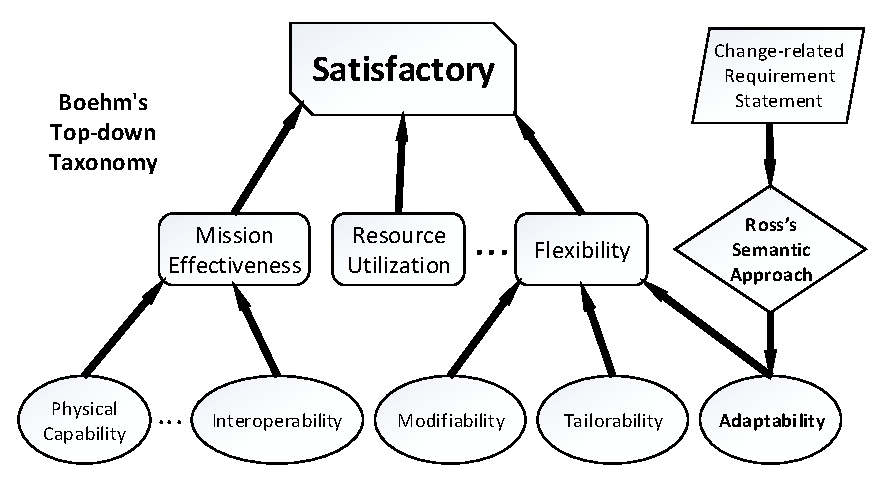
\includegraphics[scale=0.6]{img/architecture.pdf}
	\caption{Framework Architecture}
    \label{fig:arch}
\end{figure}

\subsection{Elements of Our Framework}
The elements of the specific framework that we are constructing includes: 1) hierarchies of qualities and relationships (Boehm); 2) languages for expressing specific requirements (e.g., Ross); 3) formalization of these preceding constructs; 4) integrate diverse approaches to system qualities, e.g., Boehm's top-down system quality taxonomy and Ross's bottom-up semantic approach; 5) reusable theories that can be instantiated for many projects (parameterization).

Boehm's ontology theory has been shown in the {\em Satisfactory} TypeClass. There are three level of qualities: the hight-value of a system, the second level qualities like \emph{Mission Effective} and \emph{Flexible}, and the third level contribute quality attributes like \emph{Modifiable} and \emph{Adaptable} in \emph{Flexible}. These quality attributes are organized like a taxonomy tree in our framework. The root and inside nodes of the tree are these quality attributes, and the leafs are the relations we defined to provide evidence for the lowest level of quality attributes. We deductively reason the higher level quality attributes based on lower level attributes.

In previous work, we formalized Ross's changeability requirements parser using the constructive logic of highly expressive language of the Coq proof assistant. It's a theory to define change-related qualities by extracting them from system requirement statements. We integrate Boehm's top-down theory and Ross's bottom-up theory in this framework by defining the {\em adaptability} qualities as a change statement, which is defined in our previous work \cite{Sullivan:evolutionary}.

Our framework can be parameterized by {\em System}, {\em Stakeholder}, and {\em Context}. This makes it highly generic and can be used in wide range of systems. We will give a home automation example to show how to instantiate the framework.

\subsection{Web-based Prototype Synthesis}
In order to present the theory to engineers speedily, we synthesize web-based tools form the formal specification, to let engineers use it and help find the deficiencies of our theory. If any deficiency is found, we fix it in our formal model, and then synthesize a new version of software. We use continuous deployment technique to deploy the new versions to keep this kind of iteration process in short time. This idea enable us solve the problem of concept dissemination, user-driven validation, and evolution.

\subsection{Home Automation Example}
We will give an example on how to instantiate our framework and apply it in real projects. Imagine we are building a home automation system \textbf{{\em S}}. According to Boehm's top-down theory and the interfaces that our framework provides, we first define the highest value of this system as Satisfactory. Generally, this should be the highest value of every systems. It means that all stakeholders satisfy with the systems qualities from their perspective. 

The next step is to define a system model. In our example, the system model will be defined as a unit type. The unit type is a build-in type of Coq proof assistant. It has only one value {\em tt}. We are not trying to define a complicate system model here, although it would be very interesting to study what it would be like. Our purpose here is to show how to adopt our framework in your project. Now we have a {\em Smart\_Home\_System} with type {\em unit}. We thus define a system with value {\em tt}. In order to check the qualities of this system, we still need some checkers to checker different qualities. Usually, these checkers fall in different categories. In the framework, we already encoded the taxonomy proposed by Boehm in his work of an ontology for system quality attributes \cite{Boehm:ontology}.

We then define some checkers to check the qualities we care about. In this example, we care about the physical capability, or functionality. The standard interface for the physical capability checker is like this: $physcalCapable: System->Stakeholder->Context->Prop$. To use this unified signature, we define an implementation of it. However, in order to check the specific qualities of this system. We define two check machines called {\em systemCanControlFurnaceOnOffSwitch} and {\em systemCanControlGarageDoorOpener} to provide evidence for furnace and garage door functionality perspectively. These two check machines will be called within the implementation of {\em physicalCapability} abstract function. As the code shows, the given system {\em sys} meets quality requirement of {\em physicalCapability} if it can control furnace's switch and it can control garage door opener. We can formalize more evidence for the physical capability value that we care about, and connect them with {\em conjunction} operation. There are other approaches to formalize evidence and provide check machines. That could be future work, and it's not our purpose here.

\begin{coqdoccode}
\coqdockw{Inductive} \coqdef{Example.systemCanControlFurnaceOnOffSwitch}{systemCanControlFurnaceOnOffSwitch}{\coqdocinductive{systemCanControlFurnaceOnOffSwitch}}: \coqref{Example.Smart Home System}{\coqdocdefinition{Smart\_Home\_System}} \ensuremath{\rightarrow} \coqdockw{Prop} := \coqdoceol
\coqdocindent{1.00em}
\coqdef{Example.systemCanControlFurnaceOnOffSwitch proof}{systemCanControlFurnaceOnOffSwitch\_proof}{\coqdocconstructor{systemCanControlFurnaceOnOffSwitch\_proof}}: \coqdockw{\ensuremath{\forall}} \coqdocvar{s}: \coqref{Example.Smart Home System}{\coqdocdefinition{Smart\_Home\_System}}, \coqref{Example.systemCanControlFurnaceOnOffSwitch}{\coqdocinductive{systemCanControlFurnaceOnOffSwitch}} \coqdocvariable{s}.\coqdoceol
\coqdocemptyline
\coqdocnoindent
\coqdockw{Inductive} \coqdef{Example.systemCanControlGarageDoorOpener}{systemCanControlGarageDoorOpener}{\coqdocinductive{systemCanControlGarageDoorOpener}}: \coqref{Example.Smart Home System}{\coqdocdefinition{Smart\_Home\_System}} \ensuremath{\rightarrow} \coqdockw{Prop} :=\coqdoceol
\coqdocindent{1.00em}
\coqdef{Example.systemCanControlGarageDoorOpener proof}{systemCanControlGarageDoorOpener\_proof}{\coqdocconstructor{systemCanControlGarageDoorOpener\_proof}}: \coqdocindent{-1.00em} \coqdockw{\ensuremath{\forall}} \coqdocvar{s}: \coqref{Example.Smart Home System}{\coqdocdefinition{Smart\_Home\_System}}, \coqref{Example.systemCanControlGarageDoorOpener}{\coqdocinductive{systemCanControlGarageDoorOpener}} \coqdocvariable{s}.\coqdoceol
\coqdocemptyline
\coqdocnoindent
\coqdockw{Inductive} \coqdef{Example.physicalCapability}{physicalCapability}{\coqdocinductive{physicalCapability}} (\coqdocvar{sys}: \coqref{Example.Smart Home System}{\coqdocdefinition{Smart\_Home\_System}}) (\coqdocvar{sh}: \coqref{Example.Smart Home Stakeholder}{\coqdocinductive{Smart\_Home\_Stakeholder}}) (\coqdocvar{cx}: \coqref{Example.Smart Home Context}{\coqdocinductive{Smart\_Home\_Context}}): \coqdockw{Prop} := \coqdoceol
\coqdocindent{1.00em}
\coqdef{Example.physicalCapability proof}{physicalCapability\_proof}{\coqdocconstructor{physicalCapability\_proof}}: \coqref{Example.systemCanControlFurnaceOnOffSwitch}{\coqdocinductive{systemCanControlFurnaceOnOffSwitch}} \coqdocvar{sys} \coqexternalref{:type scope:x '/x5C' x}{http://coq.inria.fr/distrib/8.4pl3/stdlib/Coq.Init.Logic}{\coqdocnotation{\ensuremath{\land}}} \coqref{Example.systemCanControlGarageDoorOpener}{\coqdocinductive{systemCanControlGarageDoorOpener}} \coqdocvar{sys} \ensuremath{\rightarrow} \coqref{Example.physicalCapability}{\coqdocinductive{physicalCapability}} \coqdocvar{sys} \coqdocvar{sh} \coqdocvar{cx}.\coqdoceol
\end{coqdoccode}

We now show how to check the adaptability value, and combine the semantic basis approach that we formalized in our previous work \cite{Dou:evolutionary} based on Ross's theory \cite{Ross:semantic}. The code snippets bellow define a value {\em smart\_home\_system\_adaptability\_requirement} of changeStatement type, which is a change related quality requirement statement. We define another check machine called {\em systemMeetsSpecificAdaptabilityRequirement} to parse the require statement to check if it is an adaptability requirement. We then implement the {\em adaptability} abstract function to call the check machine. You may notice that we do not put any evidence here to show that the system meets the {\em adaptability} requirement. But it's easy to do fulfil that. We can formalize some evidence just like in the {\em physical capability} and conjunct it with the requirement parser, and provide evidence together.

\begin{coqdoccode}
\coqdockw{Definition} \coqdef{Example.smart home system adaptability requirement}{smart\_home\_system\_adaptability\_requirement}{\coqdocdefinition{smart\_home\_system\_adaptability\_requirement}} : \coqdocrecord{changeStatement} := \coqdoceol
\coqdocindent{1.00em}
\coqdocconstructor{mk\_changeStatement} \coqdoceol
\coqdocindent{2.00em}
(\coqdocconstructor{perturbation\_shift} "some events")\coqdoceol
\coqdocindent{2.00em}
(\coqdocconstructor{context\_circumstantial} "some circumstantial contexts")\coqdoceol
\coqdocindent{2.00em}
\coqdocconstructor{phase\_preOps} \coqdoceol
\coqdocindent{2.00em}
(\coqdocconstructor{agent\_internal} "aAgent")\coqdoceol
\coqdocindent{2.00em}
(\coqdocconstructor{mk\_change} \coqdocconstructor{direction\_increase} (\coqdocconstructor{parameter\_level} "aParameter") (\coqdocconstructor{origin\_one} "anOrginin") (\coqdocconstructor{destination\_one} "aDestination") \coqdocconstructor{aspect\_function})\coqdoceol
\coqdocindent{2.00em}
(\coqdocconstructor{mechanism\_description} "some mechanism") \coqdoceol
\coqdocindent{2.00em}
(\coqdocconstructor{mk\_change} \coqdocconstructor{direction\_increase}(\coqdocconstructor{parameter\_level} "anotherParameter") (\coqdocconstructor{origin\_one} "anotherOrginin") (\coqdocconstructor{destination\_one} "anotherDestination") \coqdocconstructor{aspect\_function})\coqdoceol
\coqdocindent{2.00em}
(\coqdocconstructor{abstraction\_architecture} "anAbstraction")\coqdoceol
\coqdocindent{2.00em}
(\coqdocconstructor{valuable\_compound} "valuable because of" \coqdoceol
\coqdocindent{3.00em}
(\coqdocconstructor{reaction\_sooner\_than} 11 \coqdocconstructor{unit\_time\_second})\coqdoceol
\coqdocindent{3.00em}
(\coqdocconstructor{span\_shorter\_than} 1 \coqdocconstructor{unit\_time\_day})\coqdoceol
\coqdocindent{3.00em}
(\coqdocconstructor{cost\_less\_than} 100 \coqdocconstructor{unit\_money\_dollar})\coqdoceol
\coqdocindent{3.00em}
(\coqdocconstructor{benefit\_same\_as} "keep power off")).\coqdoceol
\coqdocemptyline
\coqdocnoindent
\coqdockw{Inductive} \coqdef{Example.systemMeetsSpecificAdaptabilityRequirement}{systemMeetsSpecificAdaptabilityRequirement}{\coqdocinductive{systemMeetsSpecificAdaptabilityRequirement}}: \coqref{Example.Smart Home System}{\coqdocdefinition{Smart\_Home\_System}} \ensuremath{\rightarrow} \coqdocrecord{changeStatement} \ensuremath{\rightarrow} \coqdockw{Prop} :=\coqdoceol
\coqdocindent{1.00em}
\coqdef{Example.systemMeetsSpecificAdaptabilityRequirement proof}{systemMeetsSpecificAdaptabilityRequirement\_proof}{\coqdocconstructor{systemMeetsSpecificAdaptabilityRequirement\_proof}}: \coqdoceol
\coqdocindent{2.00em}
\coqdockw{\ensuremath{\forall}} \coqdocvar{s}: \coqref{Example.Smart Home System}{\coqdocdefinition{Smart\_Home\_System}}, \coqdockw{\ensuremath{\forall}} \coqdocvar{c}: \coqdocrecord{changeStatement}, \coqdoceol
\coqdocindent{3.00em}
\coqexternalref{In}{http://coq.inria.fr/distrib/8.4pl3/stdlib/Coq.Lists.List}{\coqdocdefinition{In}} \coqdocconstructor{adaptability} (\coqdocdefinition{tipeAssignment} \coqdocvariable{c}) \ensuremath{\rightarrow} \coqref{Example.systemMeetsSpecificAdaptabilityRequirement}{\coqdocinductive{systemMeetsSpecificAdaptabilityRequirement}} \coqdocvariable{s} \coqdocvariable{c}.\coqdoceol
\coqdocemptyline
\coqdoceol
\coqdocnoindent
\coqdockw{Inductive} \coqdef{Example.adaptability}{adaptability}{\coqdocinductive{adaptability}} (\coqdocvar{sys}: \coqref{Example.Smart Home System}{\coqdocdefinition{Smart\_Home\_System}}) (\coqdocvar{cx}: \coqref{Example.Smart Home Context}{\coqdocinductive{Smart\_Home\_Context}}): \coqdockw{Prop} :=\coqdoceol
\coqdocindent{1.00em}
\coqdef{Example.adaptability proof}{adaptability\_proof}{\coqdocconstructor{adaptability\_proof}}: \coqref{Example.systemMeetsSpecificAdaptabilityRequirement}{\coqdocinductive{systemMeetsSpecificAdaptabilityRequirement}} \coqdocvar{sys} \coqref{Example.smart home system adaptability requirement}{\coqdocdefinition{smart\_home\_system\_adaptability\_requirement}} \ensuremath{\rightarrow} \coqdoceol
\coqdocindent{3.00em}
\coqref{Example.adaptability}{\coqdocinductive{adaptability}} \coqdocvar{sys} \coqdocvar{cx}.\coqdoceol
\end{coqdoccode} 

Overall, all the implementations of the abstract functions in the framework are like callback functions, which will be registered to the framework, and our framework will call them to check corresponding qualities. The code snippet below is a home automation instance based on our framework:

\begin{coqdoccode}
\coqdocnoindent
\coqdockw{Instance} \coqdef{Example.Smart Home Instance}{Smart\_Home\_Instance}{\coqdocinstance{Smart\_Home\_Instance}}: \coqdocclass{Satisfactory} \coqref{Example.Smart Home System}{\coqdocdefinition{Smart\_Home\_System}} \coqref{Example.Smart Home Stakeholder}{\coqdocinductive{Smart\_Home\_Stakeholder}} \coqref{Example.Smart Home Context}{\coqdocinductive{Smart\_Home\_Context}} := \{\coqdoceol
\coqdocindent{2.00em}
\coqdocmethod{sys} := \coqexternalref{tt}{http://coq.inria.fr/distrib/8.4pl3/stdlib/Coq.Init.Datatypes}{\coqdocconstructor{tt}}\coqdoceol
\coqdocnoindent
\coqdoceol
\coqdocindent{1.00em}
; \coqdocmethod{physicalCapability} := \coqref{Example.physicalCapability}{\coqdocinductive{physicalCapability}}\coqdoceol
\coqdocindent{1.00em}
; \coqdocmethod{cyberCapability} := \coqref{Example.cyberCapability}{\coqdocinductive{cyberCapability}}\coqdoceol
\coqdocindent{1.00em}
; \coqdocmethod{humanUsability} := \coqref{Example.humanUsability}{\coqdocinductive{humanUsability}}\coqdoceol
\coqdocindent{1.00em}
; \coqdocmethod{speed}:= \coqref{Example.speed}{\coqdocinductive{speed}}\coqdoceol
\coqdocindent{1.00em}
; \coqdocmethod{endurability} := \coqref{Example.endurability}{\coqdocinductive{endurability}}\coqdoceol
\coqdocindent{1.00em}
; \coqdocmethod{maneuverability} := \coqref{Example.maneuverability}{\coqdocinductive{maneuverability}}\coqdoceol
\coqdocindent{1.00em}
; \coqdocmethod{accuracy} := \coqref{Example.accuracy}{\coqdocinductive{accuracy}}\coqdoceol
\coqdocindent{1.00em}
; \coqdocmethod{impact} := \coqref{Example.impact}{\coqdocinductive{impact}}\coqdoceol
\coqdocindent{1.00em}
; \coqdocmethod{scalability} := \coqref{Example.scalability}{\coqdocinductive{scalability}}\coqdoceol
\coqdocindent{1.00em}
; \coqdocmethod{versability} := \coqref{Example.versability}{\coqdocinductive{versability}}\coqdoceol
\coqdocindent{1.00em}
; \coqdocmethod{interoperability} := \coqref{Example.interoperability}{\coqdocinductive{interoperability}}\coqdoceol
\coqdocnoindent
\coqdoceol
\coqdocindent{1.00em}
; \coqdocmethod{cost} := \coqref{Example.cost}{\coqdocinductive{cost}}\coqdoceol
\coqdocindent{1.00em}
; \coqdocmethod{duration} := \coqref{Example.duration}{\coqdocinductive{duration}}\coqdoceol
\coqdocindent{1.00em}
; \coqdocmethod{keyPersonnel} := \coqref{Example.keyPersonnel}{\coqdocinductive{keyPersonnel}}\coqdoceol
\coqdocindent{1.00em}
; \coqdocmethod{otherScareResources} := \coqref{Example.otherScareResources}{\coqdocinductive{otherScareResources}}\coqdoceol
\coqdocindent{1.00em}
; \coqdocmethod{manufacturability} := \coqref{Example.manufacturability}{\coqdocinductive{manufacturability}}\coqdoceol
\coqdocindent{1.00em}
; \coqdocmethod{sustainability} := \coqref{Example.sustainability}{\coqdocinductive{sustainability}}\coqdoceol
\coqdocnoindent
\coqdoceol
\coqdocindent{1.00em}
; \coqdocmethod{security} := \coqref{Example.security}{\coqdocinductive{security}}\coqdoceol
\coqdocindent{1.00em}
; \coqdocmethod{safety} := \coqref{Example.safety}{\coqdocinductive{safety}}\coqdoceol
\coqdocindent{1.00em}
; \coqdocmethod{reliability} := \coqref{Example.reliability}{\coqdocinductive{reliability}}\coqdoceol
\coqdocindent{1.00em}
; \coqdocmethod{maintainability} := \coqref{Example.maintainability}{\coqdocinductive{maintainability}}\coqdoceol
\coqdocindent{1.00em}
; \coqdocmethod{availability} := \coqref{Example.availability}{\coqdocinductive{availability}}\coqdoceol
\coqdocindent{1.00em}
; \coqdocmethod{survivability} := \coqref{Example.survivability}{\coqdocinductive{survivability}}\coqdoceol
\coqdocindent{1.00em}
; \coqdocmethod{robustness} := \coqref{Example.robustness}{\coqdocinductive{robustness}}\coqdoceol
\coqdocnoindent
\coqdoceol
\coqdocindent{1.00em}
; \coqdocmethod{modifiability} := \coqref{Example.modifiability}{\coqdocinductive{modifiability}}\coqdoceol
\coqdocindent{1.00em}
; \coqdocmethod{tailorability} := \coqref{Example.tailorability}{\coqdocinductive{tailorability}}\coqdoceol
\coqdocindent{1.00em}
; \coqdocmethod{adaptability} := \coqref{Example.adaptability}{\coqdocinductive{adaptability}}\coqdoceol
\coqdocnoindent
\}.\coqdoceol
\coqdocemptyline
\end{coqdoccode}

\section{Evaluation}
The evaluation goes here.

\section{Related Work}
Significant progress in these areas has been made for certain properties, particularly for system dependability properties, but not for others, such as flexibility, security, resilience, and many others. Yet the challenge in systems engineering is to produce value by achieving quality across broad ranges of system properties.

Avizienis and Laprie \cite{Laprie:dependability} informally define dependability. Their comprehensive discussion breaks dependability down into three elements: attributes, threats, and means. They proposed a taxonomy of dependability, which defines following dependability related attributes: availability, reliability, safety, integrity, and maintainability. Boehm \cite{Boehm:ontology} proposed an initial ontology for full range of system quality attributes, and argues that the value of a system is the balance of stakeholders' satisfactory. He provides a top-down taxonomy for system qualities, and studies the synergy and conflict relationships among these qualities. Ross \cite{Ross:changeability} defines a semantic basis approach for understanding the system qualities of a system, especially change-related qualities. This approach starts from the requirement statements of a system, and extract the change-related qualities. These work clarifies the nature of some system qualities, which helps us understand the role of such qualities play in evaluate the overall value of a system. But these informal theories are difficult to validate, and are hard to apply in real projects.

Assurance cases is a theory to assure the safety related attributes of a system. It asserts key requirements and properties as {\em Claims}. By using methods like testing, proofs, process, and review, people analysis, assurance case try to find the evidence that could support the claims. It then uses {\em Arguments} to show how the evidence support the {\em Claims}. Assurance cases are informally proposed as natural language. It has no tool support, and is hard to communicate. To solve the problem of poorly communication of safety arguments, Kelly \cite{Kelly:GSN} developed safety cases in graphical manner. They use graphical notations to annotate the assurance cases, and applied inductive argumentation to safety cases. 

Although there are significant researchers have been done in defining and assuring some system qualities, and some tools for engineers to use in real projects, these theories are usually expressed in informal manner, like tables and graphics, and they are hard to validate and evolve if deficiencies are found.

The overall problem in system qualities is that both of the engineering foundations and scientific foundations are weak. As to the weak engineering foundation, we have no consensus definitions for many system properties. Although some of them are well defined and studied, like dependability and safety-related, many other properties are not fully studied. We are weak in understanding of means-ends relationships among system properties, and we lack a framework for reasoning about trade-offs among system qualities. We are fundamentally weak in the ability to handle system requirements. Moreover, We have poor ability to manage full range of system qualities across system lifecycle.  As to the weak scientific foundations, we lack of rigor in research, notations, and methods employed in this area. To be specific, the research in this area are usually informal, and qualitative. The theories are generally expressed in natural language, tables and graphics. This makes the communication, reasoning, and application hard in real projects. There is no use of mathematical, computation, and logic notations critical to producing clear, unambiguous, testable theories. We also lack basis for automatically disseminate, test, validate, and to adopt and evolute of basic concepts, method, and tools. Besides, we lack rigorous and usable notations/languages for specifying the full range of system qualities that systems have to have. Except the lack of rigorous, we just have weak understanding the nature of assurance, in particular in understanding the role and interpretation of evidence and the relationship between inductive and deductive reasoning in system quality assurance.

Rushby \cite{Rushby:formalism} argues that deductive logic can play its role in safety argument. The main idea is that we can formalize the internal logic of a safety argument into deductive logic. This will provide mechanized support for assurance case argument and will help engineers focus on evidence instead of argument. Our theory steps further on this direction by providing a framework that using deductive logic as the internal logic.

Bosch \cite{Bosch:innovation} proposes an idea of innovation experiment system. In this work, he argues that the product lifecycle should be shorten to increase the customer satisfaction, and improve and quantify business gaols. The basic idea is to develop software as conducting experiments to obtain customer feedback and merge the feedback into the development process. The software development process therefore transform from waterfall model to a continuous model. We adopt the similar idea in this work by synthesizing software from the specification of our theory to enable community testing and validation. Then we fix the deficiencies founded in the testing and validation, and synthesize new software.

\section{Conclusion}
The conclusion goes here.


% use section* for acknowledgement
\section*{Acknowledgment}
The authors would like to thank...

\bibliography{mybib}{}
\bibliographystyle{plain}

% that's all folks
\end{document}


